\documentclass[a4paper,oneside,12pt,notitlepage]{article}

\usepackage[utf8]{inputenc}
\usepackage[portuges]{babel}
\usepackage{graphics}
\usepackage{palatino}
\usepackage{geometry}

\geometry{paperwidth=210mm,paperheight=297mm,
          textwidth=150mm,textheight=210mm,
          top=30mm,bottom=30mm,
          left=30mm,right=30mm}

\frenchspacing
\linespread{1.3}

\title{Lamentos de um Matemático}
\author{Paul Lockhart}
\date{}

\begin{document}

\maketitle

Um músico acorda de um terrível pesadelo.
Em seu sonho ele se encontra numa sociedade onde a educação musical tornou-se obrigatória.
``Nós estamos ajudando nossos estudantes a se tornarem mais competitivos num mundo cada vez mais cheio de sons''.
Educadores, sistemas de ensino e o Estado são os responsáveis por esse importante projeto.
Estudos foram feitos, comitês foram formados e decisões foram feitas -- tudo sem a participação de um músico ou compositor.

Como músicos são conhecidos por registrarem suas ideias em forma de partituras, esses curiosos pontos e linhas pretas devem constituir a ``linguagem da música''.
É imperativo que os estudantes tornem-se fluentes nessa linguagem se eles almejam atingir qualquer grau de competência musical;
de fato, seria ridículo esperar que uma criança cantasse ou tocasse um instrumento sem ter uma boa base de notação e teoria musical.
Tocar e escutar música ou ficar sozinho compondo uma peça original são considerados tópicos muito avançados, por isso são geralmente adiados ao menos para a graduação e mais frequentemente para a pós-graduação.

No Ensino Fundamental o objetivo é treinar os estudantes no uso dessa linguagem -- manipular símbolos de acordo com um conjunto fixo de regras:
``Aula de música é onde nós pegamos nosso caderno pautado, nosso professor coloca algumas notas no quadro e nós copiamos ou transpomos elas para um tom diferente.
Nós não podemos errar ao copiar as claves e as armaduras e nosso professor é muito exigente sobre pintar as semínimas completamente.
Uma vez tivemos um problema de escala cromática e eu acertei, mas o professor não me deu crédito porque eu coloquei as hastes no lado errado''.

No auge de sua sabedoria, os educadores logo perceberam que mesmo crianças muito novas podem receber este tipo de instrução musical.
De fato é considerado vergonhoso um garoto de terceira série não ter memorizado completamente o ciclo de quintas.
``Eu vou ter que levar meu filho a um professor particular.
Ele não se dedica aos seus deveres de música.
Diz que é chato.
Apenas senta lá, olha pela janela, cantarola para si mesmo e faz músicas bobas''.

Nas séries mais avançadas a pressão é mais forte.
Afinal, os estudantes precisam ser preparados para as tradicionais provas e para o vestibular.
Estudantes precisam ter aula de Escalas e Modos, Métrica, Harmonia e Contraponto.
``É bastante coisa pra aprender, mas depois na faculdade quando eles finalmente ouvirem tudo isso eles vão realmente apreciar o trabalho que fizeram no Ensino Médio''.
É claro que não são muitos estudantes que vão se dedicar à música, então apenas alguns irão escutar os sons que os pontos pretos representam.
De qualquer forma, é muito importante que todo membro da sociedade possa reconhecer uma modulação ou uma passagem fugal, não importa que eles nunca ouçam uma.
``Para dizer a verdade, a maioria dos estudantes não é muito boa em música.
Eles ficam entediados na sala, não tem habilidade e suas tarefas de casa são quase ilegíveis.
A maioria deles não se importa em como a música é importante no mundo de hoje;
eles apenas querem fazer o menor número possível de cursos de música pra terminar de uma vez.
Eu acho que existem pessoas que nasceram pra música e outras que não.
Eu tive uma criança que, cara, era sensacional!
Suas partituras eram impecáveis -- cada nota no lugar certo, caligrafia perfeita, sustenidos, bemóis, simplesmente lindos.
Ela será uma tremenda musicista um dia.''

Ao acordar suando frio o músico se dá conta que, felizmente, foi tudo apenas um sonho maluco.
``É claro!'' ele diz a si mesmo,
``Nenhuma sociedade reduziria uma forma de arte tão bonita e significativa para algo tão estúpido e trivial;
nenhuma cultura seria tão cruel com suas crianças a ponto de privá-las de uma expressão humana tão natural.
Que absurdo!''

Enquanto isso, do outro lado da cidade, um pintor acabara de acordar de um pesadelo semelhante\ldots

\vspace{1em}

Eu me surpreendi ao me ver numa sala de aula convencional -- sem cavaletes, sem tubos de tinta.
``Ah, nós não pintamos antes do Ensino Médio'',
me disseram os estudantes.
``Passamos a sétima série estudando cores e aplicadores''.
Eles me mostraram uma planilha.
De um lado estavam amostras de cores separadas por espaços em branco.
Eles deveriam escrever seus nomes.
``Eu gosto de pintura'',
um deles fez questão de dizer,
``me dizem o que fazer e eu faço. É fácil!''

Após a aula eu fui falar com o professor.
``Então seus estudantes não fazem nenhuma pintura?''
perguntei.
``Bem, no próximo ano eles terão Pré-Pintura-por-Números.
% Há algum termo melhor pra Paint-by-Numbers?
Isso prepara eles para o Pintura-por-Números que terão no Ensino Médio.
Então eles poderão usar o que aprenderam aqui e aplicar em situações de pintura da vida-real -- mergulhando o pincel na tinta, limpando-o, coisas assim.
É claro que nós selecionamos nossos estudantes por habilidade.
Os que são realmente excelente pintores -- aqueles que sabem suas cores e pincéis até de trás pra frente -- podem pintar um pouco mais cedo e algum deles até assistem aulas de Localização Avançada por créditos de faculdade
% Essa frase ficou estranha e deve haver uma tradução melhor que Localização Avançada. Quem puder, modifique.
% Não seriam aulas para o exame de "placement", ou seja, para validar alguma "disciplina"?
Porém, nós estamos apenas tentando dar a essas crianças uma boa base de o que é pintura, então quando eles saírem daqui para o mundo real e forem pintar sua cozinha eles não façam uma bagunça nela''.

``Hmmm, essas aulas no Ensino Médio que você mencionou\ldots{}''

``Pintura-por-números?
Nós estamos tendo muitas inscrições ultimamente.
Acho que a maioria vem por causa dos pais que querem garantir que suas crianças entrem em boas faculdades.
Nada parece melhor que Pintura-por-números Avançada num histórico de Ensino Médio''.
% Pode ser conveniente colocar uma nota de rodapé explicando como é a educação nos Estados Unidos.

``Por que as faculdades se importam com você conseguir preencher regiões numeradas com as cores correspondentes?''

``Ah, bem, você sabe, isso mostra um lúcido raciocínio lógico.
E é claro que se um estudante está planejando se formar numa ciência visual, como moda ou design de interiores, então é realmente uma boa ideia já sair do Ensino Médio com seus pré-requisitos relacionados a pintura''.

``Entendo.
E quando os estudantes podem pintar livres, numa folha em branco?''

``Você parece um de meus professores!
Eles sempre vem com essa de expressar os sentimentos e coisas desse tipo -- coisas abstratas que não tem realmente nada a ver.
% As novas normas do português eliminaram o acento de têm :)
Eu sou formado em Pintura e nunca trabalhei muito numa folha em branco.
Eu apenas uso os kits Paint-by-Numbers distribuídos pelo conselho escolar''.
% Convém revisar toda essa parte de pintura, não ficou muito boa.

\vspace{1em}

\begin{center}
***
\end{center}

\vspace{1em}

Infelizmente, nosso atual sistema de ensino de matemática é precisamente este tipo de pesadelo.
De fato, se eu tivesse que projetar um mecanismo com o propósito explícito de \textsl{destruir} a curiosidade natural de uma criança e seu prazer em criar padrões, não conseguiria fazer melhor do que está sendo feito atualmente -- eu simplesmente não teria a criatividade necessária para inventar ideias sem sentido e dolorosas como as que constituem o ensino de matemática contemporâneo.

Todos sabem que algo está errado.
Os políticos dizem, ``precisamos de padrões mais altos''.
As escolas dizem, ``precisamos de mais dinheiro e equipamentos''.
Educadores dizem uma coisa e professores dizem outra.
Estão todos errados.
As únicas pessoas que entendem o que está acontecendo são as que mais levam a culpa e são menos ouvidas: os alunos.
Eles dizem, ``a aula de matemática é inútil e chata'', e têm razão. % deve haver uma palavra melhor para "inútil" nesse contexto.

\section*{Matemática e Cultura}

A primeira coisa a entender é que matemática é uma arte.
A diferença entre matemática e as outras artes, tais como música e pintura, é que nossa cultura não a reconhece como tal.
Todos entendem que poetas, pintores e músicos criam obras de arte e se expressam por palavras, imagens e sons.
De fato, nossa sociedade é bastante generosa quando se trata de expressão da criatividade: arquitetos, chefs e até diretores de televisão são considerados artistas profissionais. % alguma sugestão melhor que "artistas profissionais"?
Porque não matemáticos?

Parte do problema é que ninguém faz a mínima ideia do quê matemáticos fazem.
O senso comum parece ser que matemáticos estão de alguma forma ligados à ciência -- talvez eles ajudem cientistas com suas fórmulas, ou digitem números enormes em computadores por uma razão ou outra.
Não há dúvida que se se o mundo tivesse que ser dividido em os ``sonhadores poéticos'' e os ``pensadores racionais'', a maioria das pessoas classificaria os matemáticos na segunda categoria.

No entanto, o fato é que não há nada tão sonhador e poético, nada tão radical, subversivo e psicodélico quanto matemática.
Ela é precisamente tão instigante quanto cosmologia ou física (matemáticos \textsl{pensaram} em buracos negros muito antes que os astrônomos encontrassem algum), e dá mais liberdade de expressão que poesia, arte ou música (que dependem fortemente de propriedades do universo físico).
A matemática é a mais pura das artes, e também a menos compreendida.

Então permitam-me tentar explicar o que é matemática, e o que os matemáticos fazem.
Provavelmente a melhor maneira é começar com a excelente descrição de G. H. Hardy:

\begin{quote}
Um matemático, como um pintor ou poeta, é um criador de padrões.
Se seus padrões são mais permanentes que os deles, é porque são feitos com \textsl{ideias}.
\end{quote}

Então matemáticos ficam fazendo padrões de ideias.
Que tipo de padrões? Que tipo de ideias?
Ideias sobre rinocerontes? Não, essas deixamos para os biólogos.
Ideias sobre linguagem e cultura? Não, normalmente não.
Essas coisas são complicadas demais para o gosto dos matemáticos em geral.
Se existe algo como um conceito estético comum na matemática, é este: \textsl{o simples é belo}.
Matemáticos gostam de pensar sobre coisas as mais simples possíveis, e as coisas mais simples são \textsl{imaginárias}.

Por exemplo, se eu estou afim de pensar sobre formas -- e eu normalmente estou -- posso pensar em um triângulo dentro de uma caixa retangular:

\begin{center}
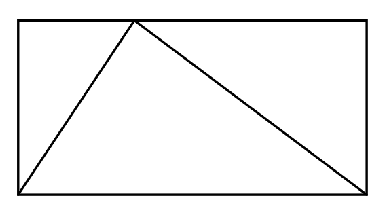
\includegraphics{triangle0.eps}
\end{center}

Eu imagino quanto da caixa o triângulo ocupa.
Dois terços, talvez?
O importante é entender que não estou falando desse \textsl{desenho} de um triângulo em uma caixa.
Nem estou falando de um objeto triangular de metal que forma as vigas de uma ponte. % alguma tradução melhor para "forming part of a girder system for a bridge"?
Não há nenhum outro propósito aqui.
Estou só \textsl{brincando}.
Isso é que é matemática -- pensar, brincar, entreter-se com sua imaginação.
A própria questão de quanto da caixa o triângulo ocupa nem faz \textsl{sentido} para objetos reais, físicos.
Até o triângulo físico feito com a maior precisão é ainda uma complicada coleção de átomos chacoalhantes; ele muda seu tamanho de uma hora para outra.
Isto é, a não ser que se queira falar sobre algum tipo de medida \textsl{aproximada}.
Bem, é aí que entra a estética.
Isto não é uma coisa simples, consequentemente é uma questão que depende de toda sorte de detalhes do mundo real.
Deixemos isso para os cientistas.
A questão \textsl{matemática} é sobre um triângulo imaginário dentro de uma caixa imaginária.
As extremidades são perfeita porque eu quero que elas sejam -- esse é o tipo de objeto sobre o qual prefiro pensar.
Este é um tema corrente em matemática: as coisas são o que você quer que sejam.
Você tem infinitas opções; a realidade não é um obstáculo.

Pelo outro lado, uma vez que tenha feito suas escolhas (por exemplo, eu posso escolher que meu triângulo seja simétrico, ou não), suas criaçõs fazem o que fazem, quer você goste, quer não.
Isto é o fascinante sobre fazer padrões imaginários: eles respondem!
O triângulo ocupa uma certa parte de sua caixa, e eu não tenho controle sobre o quanto ocupa.
Existe um número, talvez seja dois terços, talvez não, mas eu não posso dizer qual é.
Eu tenho que \textsl{descobrir} qual é.

Então podemos brincar e imaginar o que quisermos, criar padrões e fazer perguntas sobre eles.
Mas como respondemos a essas perguntas?
Não é nem um pouco parecido com ciência.
Não existe um experimento que eu possa fazer com tubos de ensaio, equipamentos e coisas do tipo que me dirá a verdade sobre um fruto da minha imaginação.
O único jeito de saber a verdade sobre nossas criações imaginárias é usando nossa imaginação, e isso é um trabalho árduo.

No caso do triângulo em sua caixa, eu vejo algo simples e belo:

\begin{center}
\includegraphics{triangle1.eps}
\end{center}

Se eu dividir o retângulo em duas partes dessa forma, posso ver que cada parte é cortada diagonalmente ao meio pelos lados do triângulo.
Então há tanto espaço dentro do triângulo quanto fora.
Isso significa que o triângulo deve ocupar exatamente metade da caixa!

É com isso que se parece um pouco de matemática. % essa frase ficou ruim, favor melhorar
Esta pequena narrativa é um exemplo da arte do matemático: fazer perguntas simples e elegantes sobre nossas invenções imaginárias, e desenvolver explicações belas e satisfatórias.
Não há realmente nada como este campo de ideias puras; é fascinante, é divertido, e é gratuito! % não sei se essa frase ficou boa...

Mas de onde surgiu essa minha ideia?
Como eu pensei em traçar aquela reta?
Como um pintor sabe onde pôr seu pincel?
Inspiração, experiência, tentativa e erro, pura sorte.
Esta é a arte do processo, criar estes pequenos e belos poemas do pensamento, estes sonetos de pura razão. % alguma palavra melhor para processo?
Há algo tão maravilhosamente transformacional nesse tipo de arte.
A relação entre o triângulo e o retângulo era um mistério, e então aquela pequena reta a tornou óbvia.
Eu não conseguia ver, mas então de repente consegui.
De alguma forma eu fui capaz de criar uma beleza profunda e simples a partir de nada, e me transformar no processo.
Não é isto a arte? % talvez melhor reescrever essa frase.

É por isso que é tão doloroso ver o que está sendo feito com a matemática na escola.
Esta rica e fascinante aventura da imaginação foi reduzida a um conjunto estéril de ``fatos'' a serem memorizados e procedimentos a serem seguidos.
Em vez de uma questão simples e natural sobre formas, e um criativo e compensador processo de invenção e descoberta, é isto que os alunos têm:

\vspace{1em}

\begin{minipage}[c]{0.45\linewidth}
	\centering
	\textbf{Fórmula da área do triângulo}

	$A=\frac12 b h$
\end{minipage}
\hspace{0.5em}
\begin{minipage}[c]{0.45\linewidth}
	\centering
	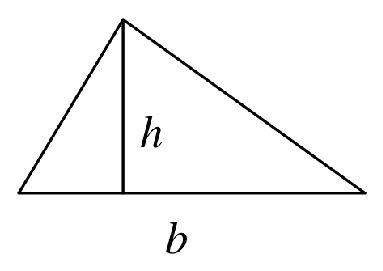
\includegraphics{triangle2.eps}
\end{minipage}

\vspace{1em}

``A área de um triângulo é igual à base vezes a altura sobre dois.''
É dito aos alunos que decorem esta fórmula e então a ``apliquem'' repetidamente nos ``exercícios''.
Foram-se a emoção, a alegria e até mesmo a dor e a frustração do ato criativo.
Não há mais nem um \textsl{problema}.
A pergunta foi feita e respondida ao mesmo tempo -- não restou nada para o aluno fazer.

% parei no início da página 5 do texto original 

\end{document}

